\documentclass[../main.tex]{subfiles}

\begin{document}
\section{Rocket Chip Configuration in the Chips System}
For the CHIPs Architecture, the Rocket Chip need to be able to direct communicate with any number accelerator. The ROCC interface was limited in its ability to communicate to an unknown number of accelerators. A private bus was added to the Rocket Chip. The Xbus was added to port list of the Rocket Chip. The Xbus connected the Rocket Chip to a unknown number of accelerators. The bus was controlled by using the custom instruction listed in the (E) extension of the RISC-V spec. This bus is a 32 bit AXI bus.

The Rocket Chip is configured to have the following features. The chip has only one tile, with an Rocket core, L1 instruction cache, L1 Data cache, ROCC accelerator (XBus controller), JTag to DMI module (For debug), no L2 cache. The chip has a 128 bit AXI bus. This bus is connected to the global shared bus (MBus). Figure \ref{fig:RocketChip} show the layout of the configured Rocket chip.
\begin{figure}
    \centering
    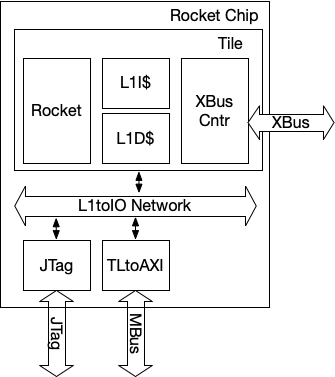
\includegraphics[scale=.5]{pngs/RocketChip.png}
    \caption{NCSU Rocket Chip}
    \label{fig:RocketChip}
\end{figure}
\end{document}